\documentclass[11pt]{article}
\newcommand{\DOCFOOT}{AMPERE POINT — automations in the Tuya app}
\newcommand{\DOCAUTH}{by Dawid Cekała}
\usepackage{fontspec}
\setmainfont{DejaVu Sans}[Scale=0.86]
\setsansfont{DejaVu Sans}[Scale=0.86]
\usepackage[a4paper,top=2.0cm,bottom=1.8cm,left=1.9cm,right=1.9cm]{geometry}
\usepackage{graphicx}
\usepackage{xcolor}
\usepackage{tikz}
\usetikzlibrary{calc}
\usepackage{enumitem}
\usepackage{fancyhdr}
\usepackage{titlesec}
\usepackage{array}
\usepackage{tabularx}
\usepackage{booktabs}
\usepackage[hidelinks]{hyperref}
\hypersetup{pdfauthor={Dawid Cekała — Ampere Point}, pdfcreator={Ampere Point}}
\usepackage{needspace}

\definecolor{apnavy}{HTML}{1A1A1A}
\definecolor{apnavy2}{HTML}{4A4A4A}
\definecolor{apink}{HTML}{1C2430}
\definecolor{apmuted}{HTML}{5B6675}
\definecolor{apline}{HTML}{E3E3E3}
\definecolor{apbg}{HTML}{F7F7F7}
\definecolor{apgreen}{HTML}{1F8A4C}
\definecolor{apgreenbg}{HTML}{E7F5EC}
\definecolor{apwarn}{HTML}{B9791B}
\definecolor{apwarnbg}{HTML}{FBF1DE}
\definecolor{apaccent}{HTML}{EC6434}

\setlength{\parindent}{0pt}
\setlength{\parskip}{0.35em}
\renewcommand{\arraystretch}{1.25}

\pagestyle{fancy}\fancyhf{}
\renewcommand{\headrulewidth}{0pt}
\renewcommand{\footrulewidth}{0pt}
\providecommand{\DOCAUTH}{oprac. Dawid Cekała}
\fancyfoot[L]{\footnotesize\color{apmuted}\DOCFOOT{} \textperiodcentered{} \DOCAUTH}
\fancyfoot[R]{\footnotesize\color{apmuted}\thepage}

% --- wordmark (placeholder do czasu otrzymania pliku logo) ---
\newcommand{\apwordmark}[1][1]{
\includegraphics[height=\dimexpr #1\dimexpr 0.86cm\relax\relax]{logo_ap.png}}

% --- pasek tytulowy ---
\newcommand{\apheader}[2]{%
\noindent\begin{tikzpicture}
  \node[anchor=north west, inner sep=0pt] at (0,0) {\apwordmark[1.15]};
\end{tikzpicture}\hfill
\raisebox{0.20cm}{\parbox[t]{9.2cm}{\raggedleft\footnotesize\color{apmuted}#2}}\\[0.25cm]
{\color{apaccent}\rule{\textwidth}{1.8pt}}\\[0.30cm]
{\fontspec{DejaVu Sans}\bfseries\color{apnavy}\LARGE #1}\\[0.15cm]}

% --- krok: numer w kolku ---
\newcommand{\kroknum}[1]{%
\tikz[baseline=(k.base)]{\node[circle, fill=apaccent, text=white, inner sep=0pt, minimum size=6.2mm,
  font=\fontspec{DejaVu Sans}\bfseries\small] (k) {#1};}}

% --- ramka informacyjna ---
\newcommand{\apinfo}[2]{%
\par\vspace{0.15cm}
\noindent\begin{tikzpicture}
\node[draw=apline, fill=apbg, line width=0.7pt, rounded corners=5pt, inner sep=8pt,
      text width=\dimexpr\textwidth-2\fboxsep-14pt\relax, align=left]
 {\small\textbf{\color{apnavy}#1}\par\vspace{2pt}\color{apink}#2};
\end{tikzpicture}\par\vspace{0.15cm}}

\newcommand{\apwarnbox}[2]{%
\par\vspace{0.15cm}
\noindent\begin{tikzpicture}
\node[draw=apwarn!45, fill=apwarnbg, line width=0.7pt, rounded corners=5pt, inner sep=8pt,
      text width=\dimexpr\textwidth-2\fboxsep-14pt\relax, align=left]
 {\small\textbf{\color{apwarn}#1}\par\vspace{2pt}\color{apink}#2};
\end{tikzpicture}\par\vspace{0.15cm}}

\newcommand{\apokbox}[2]{%
\par\vspace{0.15cm}
\noindent\begin{tikzpicture}
\node[draw=apgreen!40, fill=apgreenbg, line width=0.7pt, rounded corners=5pt, inner sep=8pt,
      text width=\dimexpr\textwidth-2\fboxsep-14pt\relax, align=left]
 {\small\textbf{\color{apgreen}#1}\par\vspace{2pt}\color{apink}#2};
\end{tikzpicture}\par\vspace{0.15cm}}

% --- komorka kroku: obrazek + opis ---
% #1 numer, #2 tytul, #3 opis, #4 plik
\newcommand{\krok}[4]{%
\begin{minipage}[t]{0.485\textwidth}
  \vspace{0pt}
  \begin{center}\includegraphics[width=\linewidth, height=7.0cm, keepaspectratio]{#4}\end{center}
  \vspace{0.12cm}
  {\kroknum{#1}\ \textbf{\color{apnavy}#2}}\par\vspace{0.05cm}
  {\small\color{apink}#3}
\end{minipage}}

\newcommand{\krokbezobrazka}[3]{%
\begin{minipage}[t]{0.485\textwidth}
  \vspace{0pt}
  \begin{center}
  
\begin{tikzpicture}
    \node[draw=apline, fill=apbg, line width=0.7pt, rounded corners=5pt, inner sep=6pt,
          minimum height=7.0cm, text width=5.3cm, align=center]
      {\footnotesize\color{apmuted}(brak zrzutu ekranu\\dla tego kroku)};
  \end{tikzpicture}
  \end{center}
  \vspace{0.12cm}
  {\kroknum{#1}\ \textbf{\color{apnavy}#2}}\par\vspace{0.05cm}
  {\small\color{apink}#3}
\end{minipage}}

% --- os czasu doby: #1 etykieta, #2 lista stref blokady "a/b,c/d"
\newcommand{\osczasu}[2]{%
\begin{tikzpicture}[x=0.62cm, y=1cm]
  \fill[apgreenbg, rounded corners=2pt] (0,0) rectangle (24,0.66);
  \foreach \a/\b in {#2}{ \fill[apwarnbg] (\a,0) rectangle (\b,0.66);
      \draw[apwarn, line width=0.8pt] (\a,0) rectangle (\b,0.66);}
  \draw[apline, line width=0.8pt, rounded corners=2pt] (0,0) rectangle (24,0.66);
  \foreach \h in {0,2,...,24}{ \draw[apline, line width=0.5pt] (\h,0) -- (\h,-0.08);
     \node[below, font=\tiny\color{apmuted}] at (\h,-0.06) {\h};}
  \node[left, font=\small\bfseries\color{apnavy}] at (-0.35,0.33) {#1};
\end{tikzpicture}}

\graphicspath{{screeny/norm/}}

\begin{document}

\apheader{Automations in the Tuya app}{How schedules and scenes work\\ Example: controlling charging hours\\ of a Wi-Fi enabled AMPERE POINT charger}

{\large\color{apink} The app gives you two different tools for controlling the charger: the schedule and automations. They look similar, but they work in completely different ways and solve different problems. This guide explains the difference, when to use which, and how to build your own rule.}

\vspace{0.35cm}
{\fontspec{DejaVu Sans}\bfseries\color{apnavy}\large Two tools, two different principles}

\vspace{0.2cm}
\begin{tabularx}{\textwidth}{@{}p{3.4cm}XX@{}}
\toprule
 & \textbf{\color{apnavy}Schedule} & \textbf{\color{apnavy}Automation (scene)}\\
\midrule
Where to find it & In the settings of the device itself & In the Smart tab $\rightarrow$ Automation\\
When it acts & At a set time & When a defined event occurs\\
What it can do & Switch on or off at a given hour & React to a change in device status\\
What it cannot do & React to anything happening between the set hours & Act on its own, without an event\\
Typical use & „Every day at 22:00, switch on” & „If charging starts at the wrong time, stop it”\\
\bottomrule
\end{tabularx}

\apinfo{The key difference}{A schedule sends a single command at the set hour and its role ends there. An automation waits for an event — it will do nothing by itself, but the moment the event occurs, it reacts immediately. This is why both are usually used together.}

\vspace{0.35cm}
{\fontspec{DejaVu Sans}\bfseries\color{apnavy}\large The problem that illustrates this}

Suppose the charger should not charge between 19:00 and 22:00. In the schedule we set: switch off at 19:00, switch on at 22:00. It looks correct — and it works, as long as the car stays plugged in throughout.

However, if the driver comes home at 19:10 and only then plugs in, charging will start. The „switch off” command was sent a quarter of an hour earlier, and plugging in the car is a new event for the charger, one that starts charging. The next command from the schedule will not arrive until 22:00.

The schedule cannot catch this, because it does not observe the device — it acts only at the set hours. What is needed is a rule that watches the device \emph{continuously}. That is exactly what an automation does.

\clearpage

% ==================== STRUCTURE ====================
\apheader{What an automation is made of}{Three elements: condition, action, time restriction}

Every automation in the Tuya app has the same structure. Understanding these three elements is enough to create your own rules.

\vspace{0.3cm}
\begin{tabularx}{\textwidth}{@{}p{2.7cm}p{3.9cm}X@{}}
\toprule
& \textbf{\color{apnavy}Element} & \textbf{\color{apnavy}Meaning}\\
\midrule
If & Condition (trigger) & The event that starts the rule. The rule „sleeps” until this event occurs.\\
Then & Action & What should happen once the condition is met.\\
Precondition & Time restriction & The window in which the rule may act at all: hours, days of the week. Outside it, the rule is inactive.\\
\bottomrule
\end{tabularx}

\apwarnbox{A precondition is not a trigger}{This is a common misunderstanding. Setting the range 19:00--22:00 does not mean „do something at 19:00”. It means „react only while the clock shows between 19:00 and 22:00”. Without the event defined in the If section, nothing will happen.}

\vspace{0.35cm}
{\fontspec{DejaVu Sans}\bfseries\color{apnavy}\large What conditions the charger offers}

After selecting the trigger \emph{When device status changes} and pointing to the charger, the app shows a list of parameters that can be watched. The most useful one is \emph{Work State} — the operating state of the device.

\vspace{0.3cm}
\begin{minipage}[t]{0.45\textwidth}
\vspace{0pt}
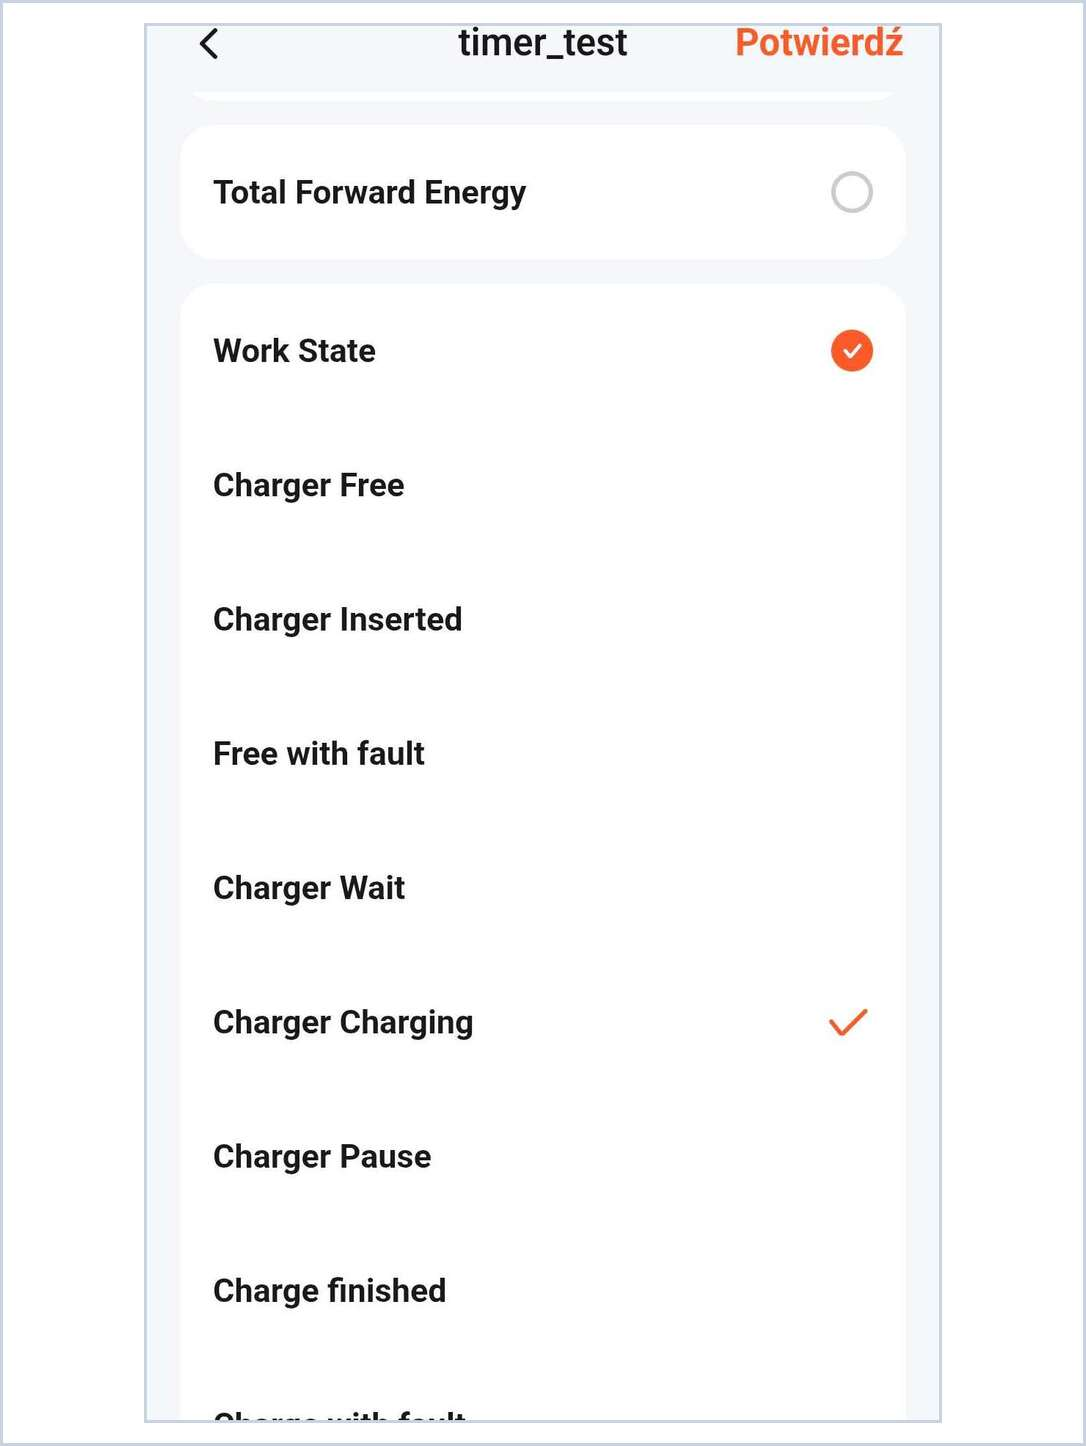
\includegraphics[width=0.84\linewidth]{s05_workstate_charging.jpg}
\end{minipage}
\hfill
\begin{minipage}[t]{0.51\textwidth}
\vspace{0pt}
\small
\begin{tabularx}{\linewidth}{@{}p{3.2cm}X@{}}
\toprule
\textbf{\color{apnavy}State} & \textbf{\color{apnavy}Meaning}\\
\midrule
Charger Free & Idle, nothing connected\\
Charger Inserted & Plug inserted into the car\\
Charger Wait & Waiting to start\\
Charger Charging & Charging in progress\\
Charger Pause & Charging paused\\
Charge finished & Charging completed\\
Free with fault & Fault with no car connected\\
Charge with fault & Fault while charging\\
\bottomrule
\end{tabularx}
\par\vspace{0.25cm}
Each of these states can act as a trigger. The rule fires the moment the charger \emph{enters} the selected state — not while it remains in it.
\end{minipage}

\clearpage

% ==================== EXAMPLE ====================
\apheader{Practical example}{Rule: „do not charge during expensive hours”\\ built step by step}

We will build a rule that stops charging started between 19:00 and 22:00, Monday to Friday. The same path applies to any other rule — only the selected values change.

\vspace{0.2cm}

\krok{1}{Create a new automation}{Smart tab $\rightarrow$ Automation $\rightarrow$ Create. If you already have other rules, use the + button in the top right corner.}{s01_automatyzacja_pusta.jpg}
\hfill
\krok{2}{Choose the trigger type}{The list contains several types. \emph{When device status changes} reacts to the device. \emph{Schedule} fires at a set hour — useful when you want to build a schedule in the form of a scene.}{s02_wybor_wyzwalacza.jpg}

\vspace{0.42cm}

\krok{3}{Point to the device}{\emph{Select a single device} picks one device. \emph{Select multiple devices} lets one rule cover several chargers at once — useful with more charging points.}{s03_device_single_warunek.jpg}
\hfill
\krok{4}{Pick the charger from the list}{The list shows all devices in the account. Devices marked as \emph{Offline} are unavailable at that moment, but can still be used in a rule.}{s04_lista_urzadzen_warunek.jpg}

\clearpage
\apheader{Practical example}{continued — condition and action}

\krok{5}{Set the condition}{Choose \emph{Work State}, then the specific state — here \emph{Charger Charging}. The rule will fire the moment charging begins.}{s05_workstate_charging.jpg}
\hfill
\krok{6}{Condition visible in the If section}{After confirming, you return to the scene screen. The condition is already saved. The rule can be extended with further conditions using +, choosing at the top whether all of them or any of them must be met.}{s06_scena_if_gotowy.jpg}

\vspace{0.42cm}

\krok{7}{Add an action}{Press + next to the Then section. Besides controlling a device, you can also run another scene, add a delay, or send a notification.}{s07_dodaj_akcje.jpg}
\hfill
\krok{8}{Point to the device to control}{It may be a different device than the one in the condition — that is the strength of scenes. Here we control the same charger, so we select it again.}{s08_device_single_akcja.jpg}

\clearpage
\apheader{Practical example}{continued — time restriction}

\krok{9}{Pick the charger}{The same device list as before.}{s09_lista_urzadzen_akcja.jpg}
\hfill
\krok{10}{Choose the parameter to change}{\emph{Switch} turns charging on and off. Also available are \emph{Charge Current Set} (current limit) and \emph{Work Mode} — so instead of stopping charging you may, for example, simply reduce the current.}{s10_switch_off.jpg}

\vspace{0.42cm}

\krok{11}{Review the complete rule}{The screen shows the condition, the action, and the \emph{Precondition} item, set by default to \emph{All day}. Without changing it, the rule would be active around the clock.}{s11_scena_if_then.jpg}
\hfill
\krok{12}{Open the time restriction}{Press \emph{Precondition}, then the validity period item. \emph{Valid When} additionally lets you make the rule depend on the state of other devices or on the weather.}{s12_precondition_calydzien.jpg}

\clearpage
\apheader{Practical example}{finishing — hours, days, saving}

\krok{13}{Choose the manual mode}{Besides manual settings, \emph{Day} and \emph{Night} modes are available, calculated from sunrise and sunset — useful for lighting, for instance. For fixed hours, choose \emph{Custom}.}{s13_czas_calydzien.jpg}
\hfill
\krok{14}{Open the hour selection}{Once manual mode is selected, a time period item appears with the default value from 00:00 to 23:59.}{s14_czas_dostosowane.jpg}

\vspace{0.42cm}

\krok{15}{Set the time range}{It is worth starting the range a few minutes before the boundary hour — the rule then begins watching before the schedule sends its command.}{s15_okres_kola.jpg}
\hfill
\krok{16}{Set days of the week and city}{Repeat selects the days. The city is needed by the app to calculate local time correctly, as well as sunrise and sunset hours.}{s16_czas_gotowy.jpg}

\clearpage
\apheader{Practical example}{finishing}

\krok{17}{Point to the city on the map}{Simply zoom to the area and confirm with OK.}{s17_miasto_mapa.jpg}
\hfill
\krok{18}{Close the settings}{The configured range is shown next to the validity period item. Press Done.}{s18_precondition_gotowy.jpg}

\vspace{0.42cm}

\krok{19}{Name the rule}{A good name contains the hours and the effect. With several rules this saves a lot of time — everything is visible in the list without opening the details.}{s19_nazwa_sceny.jpg}
\hfill
\krok{20}{Check that it is active}{The rule appears in the list with a toggle. Green means active. A rule can be switched off at any time without deleting it — useful during holidays, for example.}{s20_lista_gotowa.jpg}

\clearpage

% ==================== AUTOMATION THAT SWITCHES ON ====================
\apheader{An automation that starts charging}{A second rule: a time trigger instead of the schedule}

So far we have built a rule that \emph{stops} charging. An automation can, however, also \emph{start} it — simply choose a time trigger instead of a device state. Such a rule replaces a schedule entry and has two advantages over it.

\vspace{0.25cm}
\begin{tabularx}{\textwidth}{@{}p{5.4cm}X@{}}
\toprule
\textbf{\color{apnavy}Advantage} & \textbf{\color{apnavy}What it means}\\
\midrule
It sets the switch & The automation changes the charger's main switch, so it starts charging even when the switch was previously turned off by another rule.\\
It sets the current as a separate command & The current value is sent as an independent command, not as part of a schedule entry.\\
\bottomrule
\end{tabularx}

\apwarnbox{Why this matters}{A schedule entry that starts charging sets the device operating mode, but does not change the main switch. If the switch was turned off earlier — for example by a blocking automation or by a switch-off entry — the next schedule entry has nothing to start. The charger then has the car connected, the correct mode and the correct current, and still does not charge. The automation described on this page avoids that problem.}

\vspace{0.3cm}

\krok{1}{Create a second automation}{The same path as before: Smart $\rightarrow$ Automation $\rightarrow$ the + button in the top right corner.}{s01_automatyzacja_pusta.jpg}
\hfill
\krok{2}{Choose the time trigger}{This time not \emph{When device status changes}, but the schedule item — the rule is to act at a set hour, not in reaction to the device.}{s02_wybor_wyzwalacza.jpg}

\clearpage
\apheader{An automation that starts charging}{continued — the hour and the first action}

\krokbezobrazka{3}{Set the hour and days of the week}{Indicate when charging should start and on which days the rule applies. Set the repetition straight away — without it the rule will run only once.}
\hfill
\krok{4}{Add the first action}{Press + next to the Then section and choose device control. This rule will have two actions, not one.}{s07_dodaj_akcje.jpg}

\vspace{0.42cm}

\krok{5}{Point to the charger}{The same device list as in the previous rule.}{s09_lista_urzadzen_akcja.jpg}
\hfill
\krok{6}{Choose Charge Current Set}{The first action sets the charging current. Choose the value the charger should use — 13 A for instance. This command is sent independently of the setting in the device settings.}{s10_switch_off.jpg}

\clearpage
\apheader{An automation that starts charging}{finishing — the second action and saving}

\krok{7}{Add the second action}{Press + next to the Then section again, point to the same charger, choose \emph{Switch} and set the value to on. This is what starts charging.}{s07_dodaj_akcje.jpg}
\hfill
\krokbezobrazka{8}{Review the complete rule}{The Then section should now list two actions: setting the current and switching on. The order matters — set the current before switching on.}

\vspace{0.42cm}

\krok{9}{Name the rule}{The name should distinguish it from the blocking rule, for example „22:00 charging on 13 A”.}{s19_nazwa_sceny.jpg}
\hfill
\krokbezobrazka{10}{Check both rules in the list}{The automation list should now contain two entries: the one that starts charging and the one that blocks it, both with an active toggle.}

\apinfo{The starting rule and the blocking rule}{Both can work together, but their hours should not touch. If the block applies until 22:00, set the starting rule to 22:02. The blocking automation reacts to the start of charging within a fraction of a second, so a start exactly at the boundary hour will be interrupted by it.}

\clearpage

% ==================== RULES ====================
\apheader{Things worth remembering}{Common mistakes and proven solutions}

\vspace{0.1cm}
{\fontspec{DejaVu Sans}\bfseries\color{apnavy}\large The four most common mistakes}

\vspace{0.2cm}
\begin{tabularx}{\textwidth}{@{}p{5.0cm}X@{}}
\toprule
\textbf{\color{apnavy}Mistake} & \textbf{\color{apnavy}Consequence and how to avoid it}\\
\midrule
No days selected in the schedule & The entry runs once and then stops working. Always set the repetition.\\
Using a blocking rule to switch on & A rule reacting to the start of charging can only interrupt it. Starting requires a separate automation with a time trigger.\\
A rule without a time restriction & It will act at any hour of the day. Set the Precondition.\\
Wrong time zone on the device & All hours shift by several hours. Check it in the device settings.\\
\bottomrule
\end{tabularx}

\vspace{0.4cm}
{\fontspec{DejaVu Sans}\bfseries\color{apnavy}\large When to use a schedule, and when an automation}

\vspace{0.2cm}
\begin{tabularx}{\textwidth}{@{}p{6.6cm}X@{}}
\toprule
\textbf{\color{apnavy}Need} & \textbf{\color{apnavy}Tool}\\
\midrule
Start charging at a fixed hour & Automation with a time trigger\\
Stop charging at a fixed hour & Schedule or a time-triggered automation\\
Prevent charging during given hours, regardless of when the car is plugged in & Automation with the \emph{Charger Charging} condition\\
Reduce the current instead of stopping & Automation with the \emph{Charge Current Set} action\\
Receive a notification about a fault & Automation with the \emph{Charge with fault} condition and the \emph{Send notification} action\\
Control several chargers at once & Automation with \emph{Select multiple devices}\\
\bottomrule
\end{tabularx}

\apinfo{Internet connection}{The schedule is stored in the device itself and, once saved, works without internet access as well. Automations are executed in the cloud and require a connection. After a longer power outage the device may need to synchronise with the app again in order to restore the saved hours. If controlling the current matters to you, choose an automation — the schedule does not always pass the current value correctly.}

\apokbox{The most reliable solution technically}{If control over charging hours is to be entirely dependable, it is worth setting a schedule in the car as well. The vehicle then draws no power outside the defined hours regardless of the app, the charger and the internet connection.}

\vspace{0.5cm}
{\color{apline}\rule{\textwidth}{0.8pt}}\\[0.15cm]
{\footnotesize\color{apmuted} If you have any questions, please contact us: hello@amperepoint.com}

\end{document}
